\documentclass{article}
\usepackage[utf8]{inputenc}
\usepackage{listings}

\title{MS Azure Notes}
\author{Mark Potter}
\date{January 2021}

\usepackage{natbib}
\usepackage{graphicx}

\newcommand{\code}{\texttt}

\begin{document}

\maketitle

\begin{abstract}
This document serves as an accompaniment to the learning paths provided by Microsoft for working towards the AZ-204 exam. It may also be of interest to anyone looking for an overview of development on the Azure platform generally.
\end{abstract}

\section{Introduction}
These are notes I compiled while working through the learning paths for The Microsoft Azure Developer Certification AZ-204 in early 2021. I aim to keep the notes in line with the structure of the leaning paths at this time. 

\section{Create Serverless Apps}

This section lays out the serverless services offered by the Azure platform and walks you through creating Azure Functions. The learning path focuses predominately on using the Azure Portal to create functions however I opted to use Visual Studio Code (VSC) for most of the development. Instructions for setting up your development environment are covered by the learning path.

\subsection{Choose the best Azure service to automate your business processes}
Here we are introduced to four workflow implementation technologies:
\begin{itemize}
    \item Logic Apps
    \item Microsoft Power Automate
    \item WebJobs
    \item Azure Functions
\end{itemize}

they all \textbf{accept inputs}, \textbf{perform actions}, \textbf{support conditions} and \textbf{return outputs}.

These technologies fall into two categories: \textbf{design-first} technologies and \textbf{code first} technologies, with Logic Apps and MS Power Automate being design-first and WebJobs and Azure Functions being code-first. Design-first technologies let you create workflows with flow diagrams whereas code-first technologies require programming. 

\begin{figure}[h!]
\centering
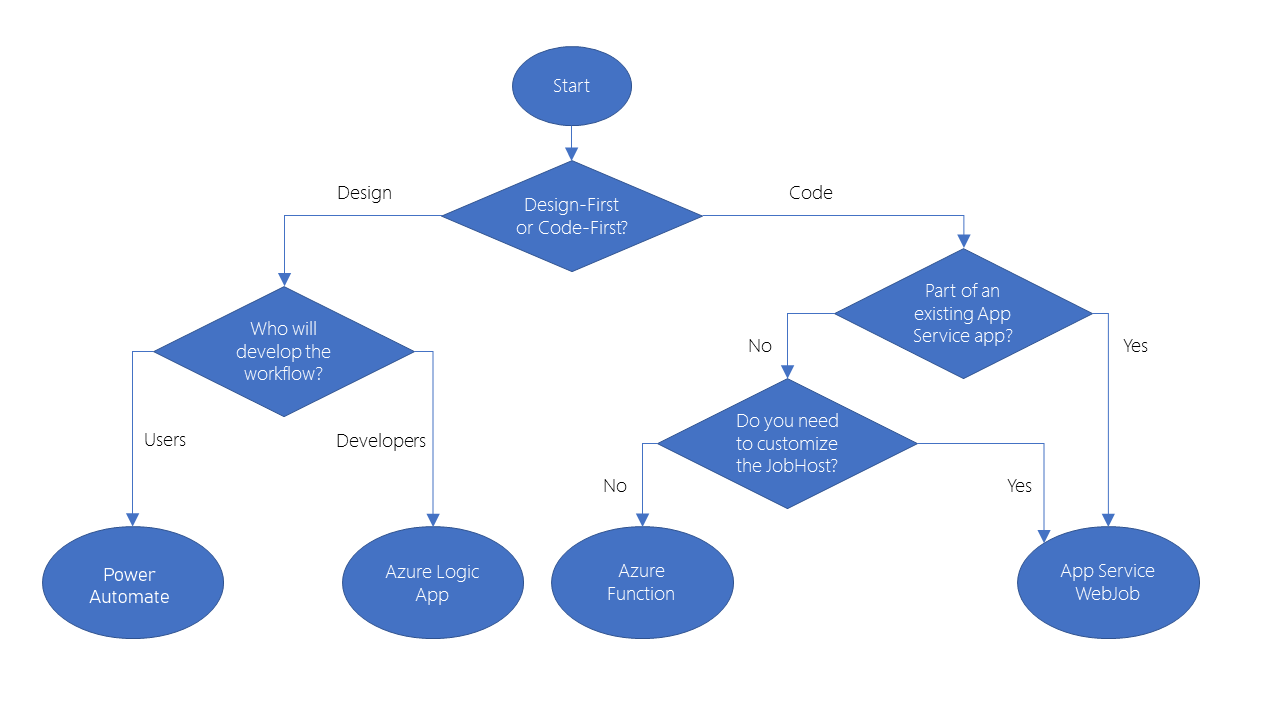
\includegraphics[scale=0.35]{service-choice-flow-diagram}
\caption{Decision tree for choosing a workflow implementation technology.}
\label{fig:service-choice-flow-diagram}
\end{figure}

\subsubsection{Logic Apps}
Logic apps can be created with either the flow diagram GUI or by writing your own JSON describing the workflow. Logic apps have \textbf{connector} components which let you interface with external services. There are over 200 builtin connectors and you can write your own. Logic apps are aimed at developers but are useful in situations where clear communication of what the workflow does is important to \textbf{non-technical} stakeholders. 

\subsubsection{Microsoft Power Automate}
MS Power Automate is similar to Logic Apps but is intended to be used by \textbf{non-technical} users. It works with a similar flow diagram style GUI but with no support for defining your own JSON. You can still create custom connectors and under the hood it's still just a Logic App.

\subsubsection{WebJobs}
WebJobs come in two flavours \textbf{continuous} and \textbf{triggered}. They can be written in a wide range of languages however the SDK only supports C\#. Using the SDK provides access to \code{JobHostConfiguration} and \code{HostBuilder} which let you interact the the Azure App Service 

\subsubsection{Azure Functions}
Azure functions only use resources when the function code is being run. They start in response to a \textbf{trigger}, all Azure functions have one. Example triggers are HTTP calls, timers or documents added to a database collection. You can create Azure Functions in the Azure Portal or in VSC. They should be your \textbf{default choice} when taking the code-first approach.

\subsection{Create serverless logic with Azure Functions}
Serverless compute is great because you don't have to manually provision infrastructure. You don't have to worry about over allocating resources as \textbf{instances are created and destroyed on demand}. However there are some instances in which Azure Functions may not be the best option. Azure Functions have a \textbf{maximum timeout of ten minutes} (two and half for functions invoked by HTTP). There's also a limit on scaling, you can only spawn \textbf{200 concurrent instances} of a function app and you can only \textbf{provision a new one every ten seconds}. \textit{N.B} One function app instance can service multiple requests so while there is no set limit to how much traffic an instance can handle it may be cheaper to host your service on a VM.

\subsubsection{Create a function app}
This section of the learning path walks you through creating a function app in the Azure Portal. You just need to fill in a few inputs in a form and the portal takes care of the rest. You'll get some example code which you can run and rewrite in the portal if you want to have a play. You can also make requests to the function's endpoint which you can reveal by clicking "Get function URL". cURL and Postman are good tools for this. You can also check the monitoring dashboard to see requests made to your function. This section also introduces the \code{context} object. Those using JavaScript will notice that in the default function code \code{context.log} is used where they might expect to see \code{console.log}. While \code{console.log} will not error in newer versions of the function app runtime it's use is discouraged because a \textbf{\code{console.log} will not be tied to a specific invocation of your function}. 

\subsubsection{Secure HTTP triggers}
When creating an HTTP triggered function you'll be asked to select an authorisation level. The Admin level will require your master key, the function level uses function keys which are scoped to this particular function, the anonymous level required no authorisation. To provide auth when making a request to your function you can either include your key with the query param \code{code} (\textit{eg} \code{https://my-app.azurewebsites.net/api/myFunc?code=<key>}) or by including an \code{x-functions-key} header with your request.

\subsection{Execute an Azure Function with triggers}
There are a bunch of events that can be used as triggers for functions. This section covers the use of HTTP (as seen in the last section), timers and blobs. 

Timer triggers are very simple to configure, all they need is a NCRONTAB expression to tell them when to run. NCRONTAB is just like CRON but with a sixth figure at the start representing seconds. Your function will be passed an instance of the timer object as an argument. The timer object has an \code{isPastDue} property which is boolean and does what it says on the tin. 

Blob triggers are kicked off when a blob is added to a given storage container. You can configure your function to only trigger if the blob has a specific extension by adding the extension to the trigger's path (defined in \code{function.json}) \textit{eg} \code{blob-store/\{blobName\}.zip} will trigger the function only if a zip file is uploaded. The blob that triggers your function will be available as an argument however I would recommend accessing it via \code{context.bindings} despite Microsoft's recommendation. The arguments of your function (after \code{context}, of course) will be your functions bindings (trigger, inputs and outputs) in order of their appearance in \code{function.json}. Therefore, in my opinion, consuming the bindings as arguments is a significantly more flimsy approach than destructuring \code{context.bindings}, \textit{eg}

\begin{lstlisting}
const { 
    timerTrigger, 
    blobInput, 
    httpOutput 
} = context.bindings
\end{lstlisting}

\subsection{Chain Azure Functions together using input and output bindings}
In this section we learn a bit more about inputs and outputs, nothing too dramatic. Inputs let you read from data sources like databases, blob storage or queues. You can attach many inputs to one function. Your function will read from these when it is invoked but it will not be invoked because them; remember your function can only have one trigger. Outputs can also be numerous and similarly can be things like database operations or HTTP responses. This implies that Azure Functions can be chained. As an example imagine a user uploads a profile picture to our social network. We place the file directly into a blob store which triggers our first function. This function writes a reference to the blob to our databases users table and adds the blob to a message queue. A second function is triggered by the blob being added to a queue and produces a thumbnail for us and outputs it to the blob store where it's picked up by a third function which again writes to the users table. 

Define a binding as an output or an input by specifying the \code{direction} parameter in \code{function.json} as \code{in} or \code{out}. Some bindings can take additional parameters \textit{eg} CosmosDB can be given an \code{id} parameter which it will use when being asked to find, update or insert a document, but you can also provide an \code{sqlQuery} parameter if you need to retrieve multiple documents. 

\subsection{Create a long-running serverless workflow with Durable Functions}
Durable functions let us use serverless environments but with the added advantage of a state which is maintained between functions. Durable functions are great for scenarios where the workflow relies on 
external events which may take some time, like a manual approval step by a human.

The stateful workflow of a durable function is defined by its \textbf{orchestration function}. The orchestration function can handle synchronous and asynchronous function calls letting you save the results locally as variables. Azure will add a checkpoint when the orchestrator awaits, it may then choose to dehydrate until the wait is completed, at which point it will rehydrate. You don't need to add any code to do this, its baked in for you.

Durable functions are made up of Azure Functions. The literature refers to three distinct types: Orchestrator functions which hold the overall state of the workflow, client functions which are the entry point which runs in response to a trigger and activity functions which is where the actual work done by the durable function should be. 

To write durable functions you'll need the durable-functions npm package. This package contains not only the orcestrator itself but also functions such as \code{callActivity} (where a checkpoint will be added) and \code{createTimer} (which you should use instead of \code{setTimeout} or \code{setInterval}).
When you make a request to an orchistrator you'll get back a 202 status and a piece of JSON with several URIs. making a GET request to the \code{statusQueryGetUri} will yield more JSON which let's you know about the internal state of the durable function.

\subsection{Monitor GitHub events by using a webhook with Azure Functions}
This section goes through setting up an HTTP triggered Azure Function and configuring a GitHub webhook. It's pretty easy going, the only think I'll mention here is the security. You'll need to made your function security level anonymous and check the secret given in the request from GitHub yourself. The recommended method to do this is to make a sha1 hash of the key you provided as a secret to GitHub and prepend the string \code{'sha1='}. You can then compare the result directly to the \code{x-hub-signature} header on the request, returning a 401 code if you don't get a match.

\subsection{Enable automatic updates in a web application using Azure Functions and SignalR Service}
Polling is inefficient. If you use polling you'll be making requests whether or not there is any new data to display and the data you are displaying could be a whole polling interval behind the actual data. The workaround proposed is SignalR. 

SignalR creates persistent connections between client and server allowing us to push updates when they happen. This is great because we can exploit an Azure Function triggered by changes in a CosmosDB to push the updates. At time of writing SignalR's preferred transport is WebSockets, however if they aren't available it will fall back to Server Sent Events or Ajax long polling. We get future proofing as when a new technology replaced WebSockets we won't need to update anything except for SignalR. 
To get setup create one Azure Function to "negotiate" the SignalR connection and another to broadcast changes. The negotiator is triggered by HTTP and takes a SignalR connection as an input, whcih it then returns via HTTP. The broadcaster is triggered by CosmosDB documents and outputs to SignalR. The broadcaster needs to reformat the updates it receives as input but this can be done with a simple map.

\begin{lstlisting}
module.exports = async function (context, documents) {
    const updates = documents.map(stock => ({
        target: 'updated',
        arguments: [stock]
    }));

    context.bindings.signalRMessages = updates;
    context.done();
}
\end{lstlisting}

\subsection{Expose multiple Azure Function apps as a consistent API by using Azure API Management}
Azure API Management lets us assemble many small APIs into one big API. It also takes a bunch of headache out for us by handling "request authentication and authorization, rate limit and quota enforcement, request and response transformation, logging and tracing, and API version management." API Management can be set up without leaving the function app portal experience. Managed APIs will be hosted on the azure-api.net domain as opposed to the azurewebsites.net domain where function apps are hosted.

Microservices can present challenges such as services being presented under disparate addresses, replying in different formats or having different security implementations. API Management addresses this by letting us change microseverice definitions and locations without updating client apps, presenting a single URI for all our services, enforcing consistent formats and security rules.

Access to your managed API is controlled by Subscriptions. Subscriptions provide keys to be attached as \code{ocp-apim-subscription-key} headers in requests.
\end{document}
